\documentclass{beamer}

\mode<presentation> {

%\usetheme{default}
%\usetheme{AnnArbor}
%\usetheme{Antibes}
%\usetheme{Bergen}
%\usetheme{Berkeley}
\usetheme{Berlin} %+
%\usetheme{Boadilla}
%\usetheme{CambridgeUS} %-
%\usetheme{Copenhagen}
%\usetheme{Darmstadt}
%\usetheme{Dresden}
% \usetheme{Frankfurt} %+
%\usetheme{Goettingen}
%\usetheme{Hannover}
%\usetheme{Ilmenau}
%\usetheme{JuanLesPins}
%\usetheme{Luebeck}
% \usetheme{Madrid}      
%\usetheme{Malmoe}
%\usetheme{Marburg}
%\usetheme{Montpellier}
%\usetheme{PaloAlto}
%\usetheme{Pittsburgh}
% \usetheme{Rochester} %min
% \usetheme{Singapore}
%\usetheme{Szeged}
%\usetheme{Warsaw}

% As well as themes, the Beamer class has a number of color themes
% for any slide theme. Uncomment each of these in turn to see how it
% changes the colors of your current slide theme.

%\usecolortheme{albatross}
%\usecolortheme{beaver}
%\usecolortheme{beetle}
%\usecolortheme{crane}
%\usecolortheme{dolphin}
%\usecolortheme{dove}
% \usecolortheme{fly}
%\usecolortheme{lily}
%\usecolortheme{orchid}
% \usecolortheme{rose}
% \usecolortheme{seagull}
%\usecolortheme{seahorse}
\usecolortheme{whale}
%\usecolortheme{wolverine}

%\setbeamertemplate{footline} % To remove the footer line in all slides uncomment this line
%\setbeamertemplate{footline}[frame number] % To replace the footer line in all slides with a simple slide count uncomment this line

\setbeamertemplate{navigation symbols}{} % To remove the navigation symbols from the bottom of all slides uncomment this line

\setbeamercovered{transparent} % Fait apparaître les animations en grisé (utile pour la conception, mais peut être commenté lors de la remise du document final)

% Pour utiliser une police à empattements partout
\usefonttheme{serif}

% Pour rajouter la numérotation des frames dans les pieds de page
\newcommand*\oldmacro{}%
\let\oldmacro\insertshorttitle%
\renewcommand*\insertshorttitle{%
  \oldmacro\hfill%
  \insertframenumber\,/\,\inserttotalframenumber}

}

% для нумерации картинок
\setbeamertemplate{caption}[numbered]


\setbeamertemplate{headline}
{%
  % \begin{beamercolorbox}[colsep=1.5pt]{upper separation line head}
  % \end{beamercolorbox}
  \begin{beamercolorbox}{section in head/foot}
    \vskip0pt\insertnavigation{\paperwidth}\vskip2pt
  \end{beamercolorbox}%
  % \begin{beamercolorbox}[colsep=1.5pt]{lower separation line head}
  % \end{beamercolorbox}
}

\usepackage[T2A]{fontenc}
\usepackage[utf8]{inputenc}
\usepackage[english]{babel}
\usepackage{hyperref}     % ТАК_НУЖНО
\hypersetup{unicode=true} % ТАК_НУЖНО
\usepackage{amsmath}
\usepackage{amssymb,textcomp, esvect,esint}
\usepackage{amsfonts}
\usepackage{amsthm}
\usepackage{graphicx}
\usepackage{indentfirst}
\usepackage{xcolor}
% \usepackage{enumitem} %--- ломал нумерацию!?

\usepackage{graphicx}
\usepackage{booktabs}
\usepackage{caption}
\usepackage{listings}
\usepackage{tikz}
\usepackage{xcolor}



\usepackage{media9}
\usepackage{animate}
\usepackage{threeparttable}
\usepackage{pifont}


\usepackage{import}
\usepackage{xifthen}
\usepackage{pdfpages}
\usepackage{transparent}

\usepackage[skip=1pt]{caption}
% add (renew) commands

\renewcommand{\Im}{\mathop{\mathrm{Im}}\nolimits}
\renewcommand{\Re}{\mathop{\mathrm{Re}}\nolimits}

\renewcommand{\d}{\, d}
\renewcommand{\leq}{\leqslant}
\renewcommand{\geq}{\geqslant}
\renewcommand{\l}{\left}
\renewcommand{\r}{\right}

\newcommand{\vc}[1]{\mbox{\boldmath $#1$}}
\newcommand{\T}{^{\text{T}}}


\newcommand{\diag}{\mathop{\mathrm{diag}}\nolimits}
\newcommand{\cl}{\mathop{\mathrm{cl}}\nolimits}
\newcommand{\grad}{\mathop{\mathrm{grad}}\nolimits}
\renewcommand{\div}{\mathop{\mathrm{div}}\nolimits}
\newcommand{\rot}{\mathop{\mathrm{rot}}\nolimits}
\newcommand{\Ker}{\mathop{\mathrm{Ker}}\nolimits}
\newcommand{\Spec}{\mathop{\mathrm{Spec}}\nolimits}
\newcommand{\sign}{\mathop{\mathrm{sign}}\nolimits}
\newcommand{\tr}{\mathop{\mathrm{tr}}\nolimits}
\newcommand{\rg}{\mathop{\mathrm{rg}}\nolimits}


\newcommand{\DS}{\mathcal D\left(\mathbb{R}\right)}
\newcommand{\QED}{\textnormal{Q. E. D.}}
\newcommand{\dseq}{\overset{\mathcal D'}{=}}
\newcommand{\dto}{\overset{\mathcal D'}{\to}}


\newcommand{\const}{\text{const}}
\newcommand{\xmark}{\ding{55}}


\newenvironment{uproof}{
% \begin{comment}
\par \color{ugray}
\begin{proof}[$\triangle$]
}{
\end{proof} \par
% \end{comment}
}


\newcommand{\bhat}{\overset{\text{\scalebox{0.8}[0.5]{\rotatebox[origin=c]{180}{$\wedge$}}}}}

\newcommand{\cf}[1]{\text{\raisebox{1.5pt}{$\scalebox{1.3}{$\chi$}$}}_{#1}}

\newcommand{\supp}{\mathop{\mathrm{supp}}\nolimits}
\newcommand{\si}{\mathop{\mathrm{Si}}\nolimits}

\newcommand{\rr}{\rightrightarrows}

% \newcommand{\sbsnum}[2]{
%     \setcounter{subsection}{\the\numexpr #1 - 1 \relax}
%     \subsection{#2}
% }

% Секции и сабсекции
% \definecolor{darkblue}{HTML}{000099}
% \newcommand{\sbs}[1]{\subsection{\textcolor{darkblue}{#1}}}
% \renewcommand{\sec}[1]{\section{\textcolor{darkblue}{#1}}}
\newcommand{\sbs}[2]{
\setcounter{subsection}{\numexpr #1 - 1 \relax}
    \textcolor{ugreen}{
        \subsection{#2}
        }
}


% \newcommand{\progressbar}{%
	\pgfmathsetmacro{\slidewidth}{\paperwidth}
	\pgfmathsetmacro{\progressstep}{\paperwidth/\inserttotalframenumber}
	\pgfmathsetmacro{\progresspos}{(\insertframenumber - 0.5) * \progressstep}
	\begin{tikzpicture}[scale = 0.035, line width = 1ex]
		\node[inner sep=0pt] (cat) at (\progresspos,0)	{
\includegraphics[width=30pt]{settings/cat.png}};
		\path[red] (0,0) -- (\slidewidth,0);
	\end{tikzpicture}
}

\makeatletter
\setbeamertemplate{footline}
{
\hfill \progressbar%
  \leavevmode%
  \hbox{%
  \begin{beamercolorbox}[wd=.433333\paperwidth,ht=2.25ex,dp=1ex,center]{section in head/foot}%
    \usebeamerfont{author in head/foot}\insertshortauthor~~\beamer@ifempty{\insertshortinstitute}{}{(\insertshortinstitute)}
  \end{beamercolorbox}%
  \begin{beamercolorbox}[wd=.333333\paperwidth,ht=2.25ex,dp=1ex,center]{section in head/foot}%
    \usebeamerfont{title in head/foot}\insertshorttitle
  \end{beamercolorbox}%
  \begin{beamercolorbox}[wd=.333333\paperwidth,ht=2.25ex,dp=1ex,right]{section in head/foot}%
    % \usebeamerfont{date in head/foot}\insertshortdate{}\hspace*{2em}
    % \insertframenumber{} / \inserttotalframenumber\hspace*{2ex} 
  \end{beamercolorbox}}%
  \vskip0pt%
}

\setbeamertemplate{caption}[numbered]

\title[Optical chaos]{Literature review on topic \\ <<Chaos optical communication>>}
\author{Eskoskin D., Khoruzhii K., Primak E.}
\institute[MIPT]

\begin{document}
\date{05.03.2021}
\maketitle

% \setlength{\abovedisplayskip}{3pt}
\setlength{\abovedisplayshortskip}{3pt}
\setlength{\belowdisplayskip}{3pt}
\setlength{\belowdisplayshortskip}{3pt}

% \AtBeginSection[]
% {
    % \begin{frame}
    %     \frametitle{Table of Contents}
    %     \tableofcontents
    % \end{frame}
% }

% подключаем слайды внутри соответствующих файлов:
% \frame{
... \frametitle{TITLE}}
\frame{
With $\lambda/4$ plate added we can observe the color change when rotating the base of the arrow holder.

\phantom{42}


\begin{minipage}{0.3\textwidth}
    \begin{figure}[h]
    \flushleft
    \vspace{-5mm}
    \animategraphics[loop,controls=play,width=1.0\textwidth]{10}{gifs/g6/}{1}{152} 
    \end{figure}
\end{minipage}
\hfill
\begin{minipage}{0.65\textwidth}
We coud get mean value of rgb color.


It would be interesting to look at RGB in HSV terms. 

\phantom{42}

There are several references to the possibility, in some assumptions to restore wavelength on HSV decomposition.
    \begin{figure}[h]
        \centering
        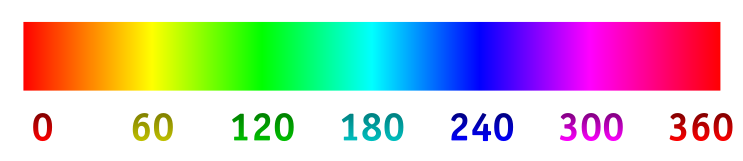
\includegraphics[width=1\textwidth]{figures/HueScale.png}
        % \vspace{-14mm}
        \caption{Hue in the HSV encodings of RGB}
    \end{figure}
\end{minipage} \frametitle{TITLE}}
\frame{
\begin{itemize}
	\item the observation of polarization phenomenon;

	\phantom{239}

	\item studing the methods of getting a polarized light;

	\phantom{239}

	\item looking at the aspects of polarization and some magic.
\end{itemize}	\frametitle{Our aims in this work}
}

\section{Mirror}

\frame{
\begin{minipage}{0.55\textwidth}
    \begin{figure}[h]
    \centering
    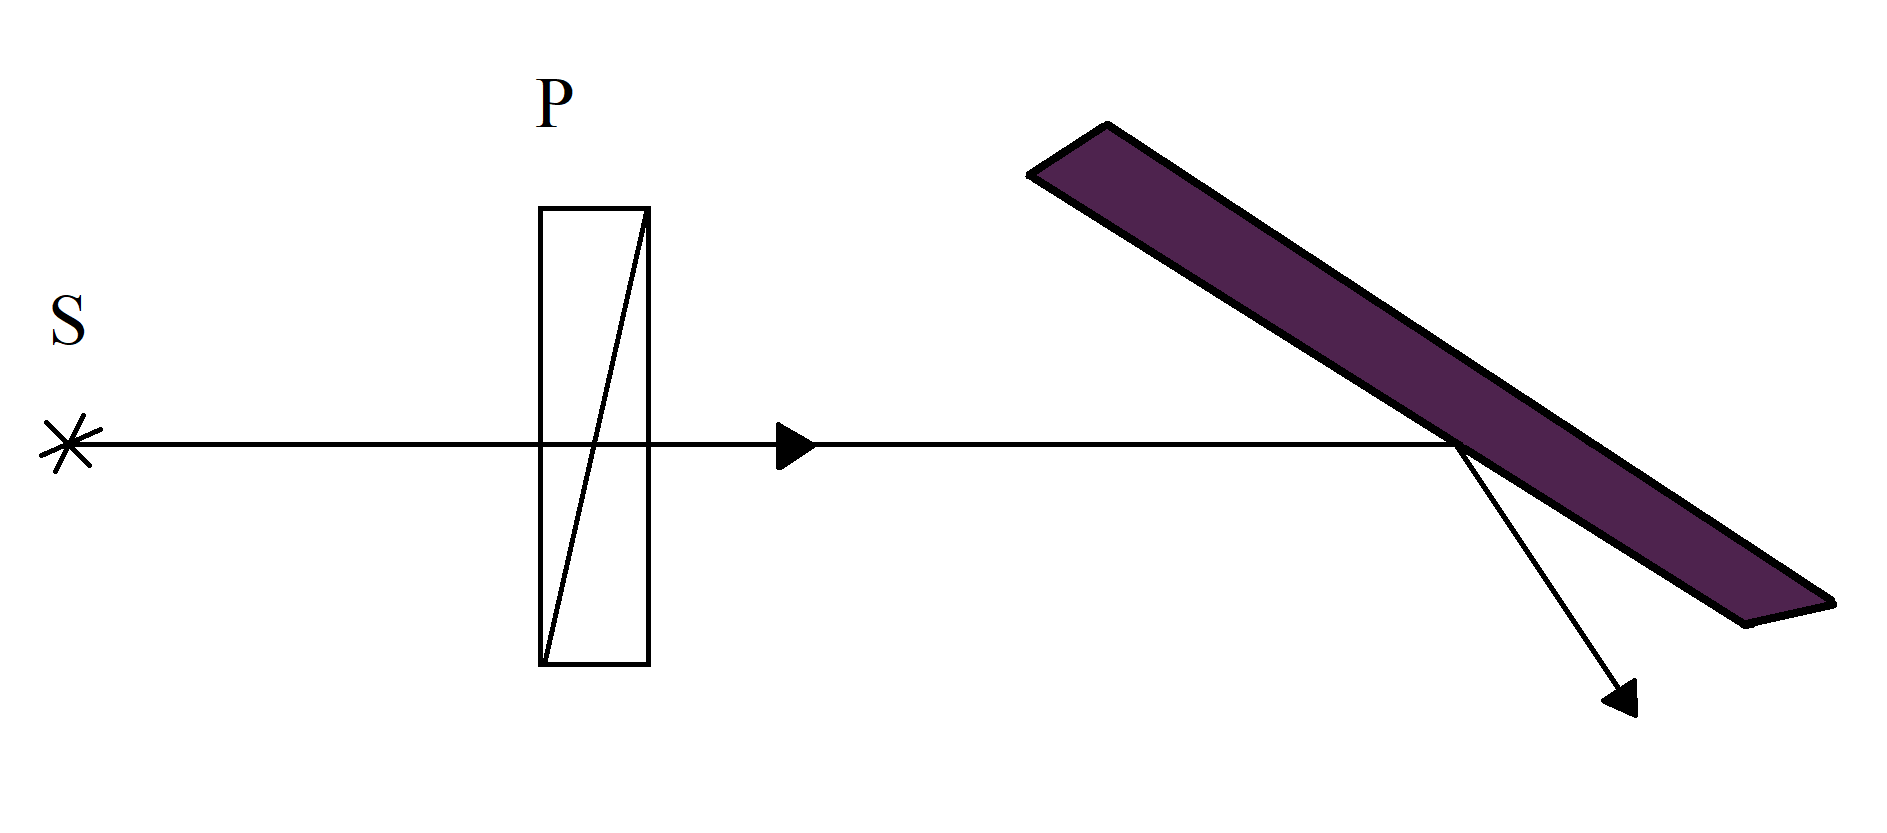
\includegraphics[width=1\textwidth]{images/mirror.png}
    \caption{We put a polaroid P and a mirror (violet one) on the way of light.}
    %\label{fig:}
\end{figure}
\end{minipage}
\hfill
\begin{minipage}{0.35\textwidth}
	Now we can make a rough estimation of polarization direction. And by adding the second polaroid we can also etimate it's polarization direction.
	\begin{align*}
		&P_1 \colon -4^\circ&\\
		&P_2 \colon 291^\circ&
	\end{align*}
\end{minipage}

	\frametitle{The experiment setup}
}
\frame{
\begin{minipage}{0.45\textwidth}
    \begin{figure}[h]
    \centering
    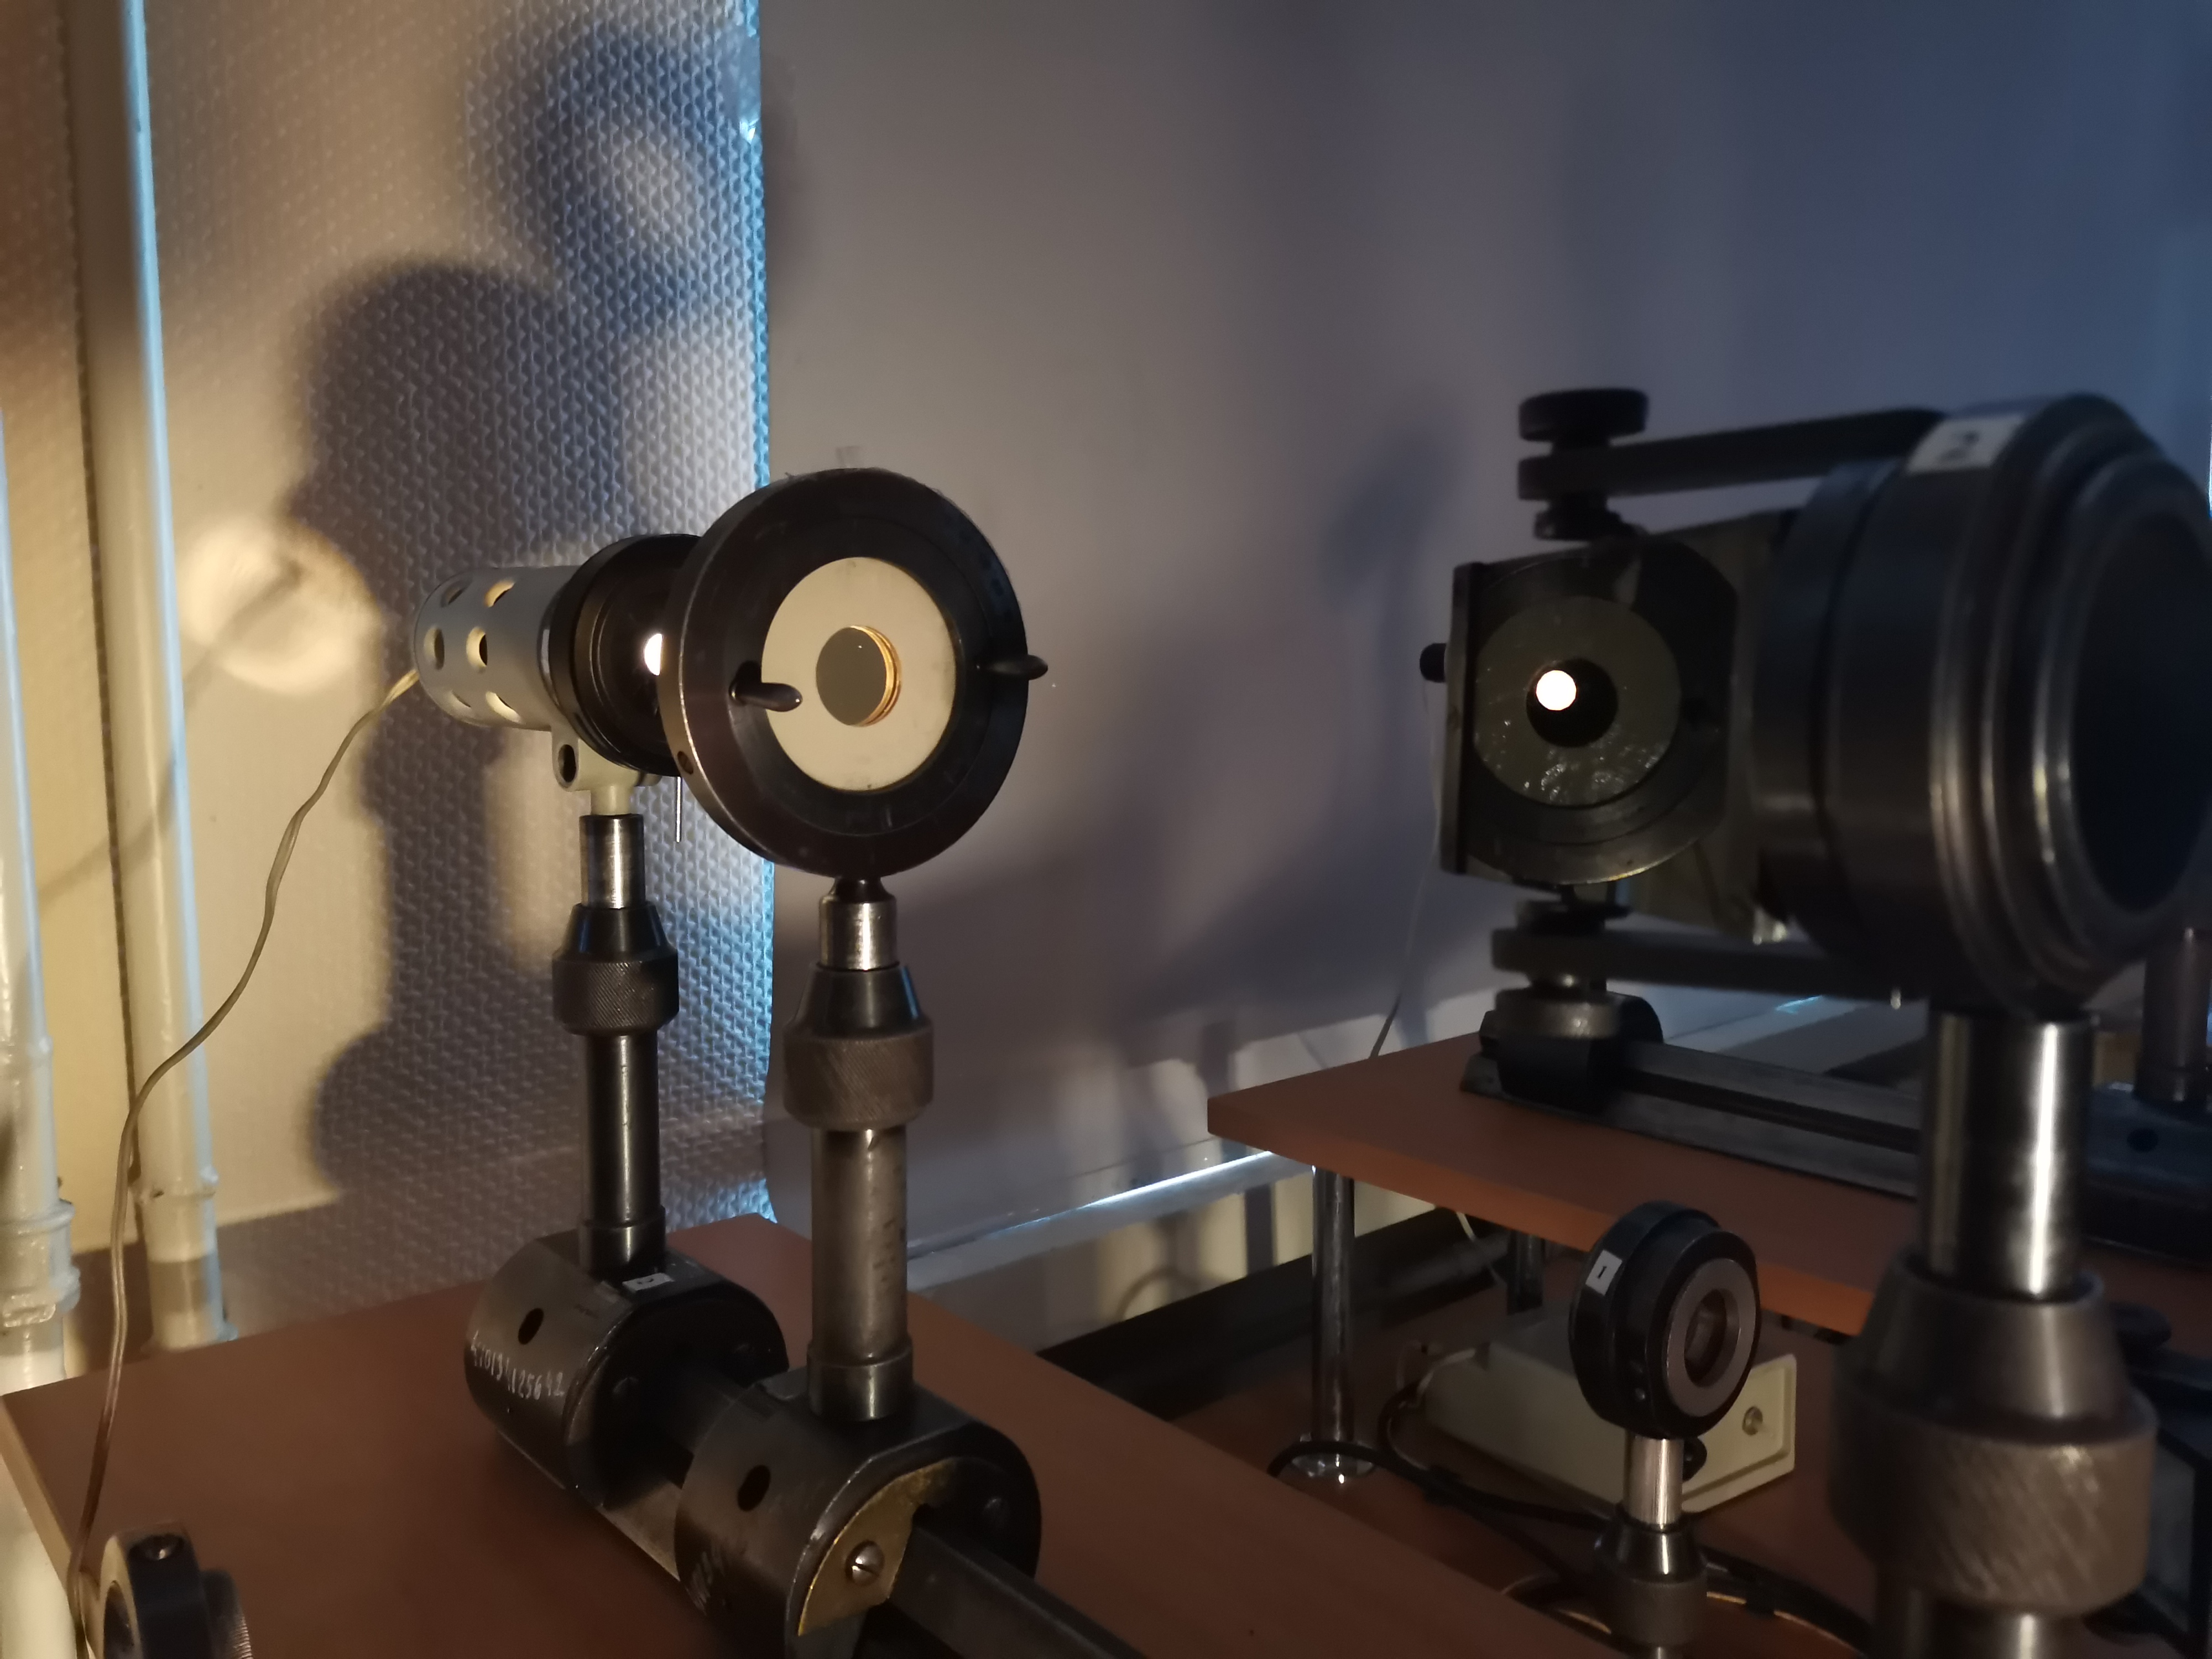
\includegraphics[width=1.1\textwidth]{images/mirror-pol.jpg}
    \caption{With the mirror.}
	\end{figure}
\end{minipage}
\hfill
\begin{minipage}{0.45\textwidth}
    \begin{figure}[h]
    \centering
    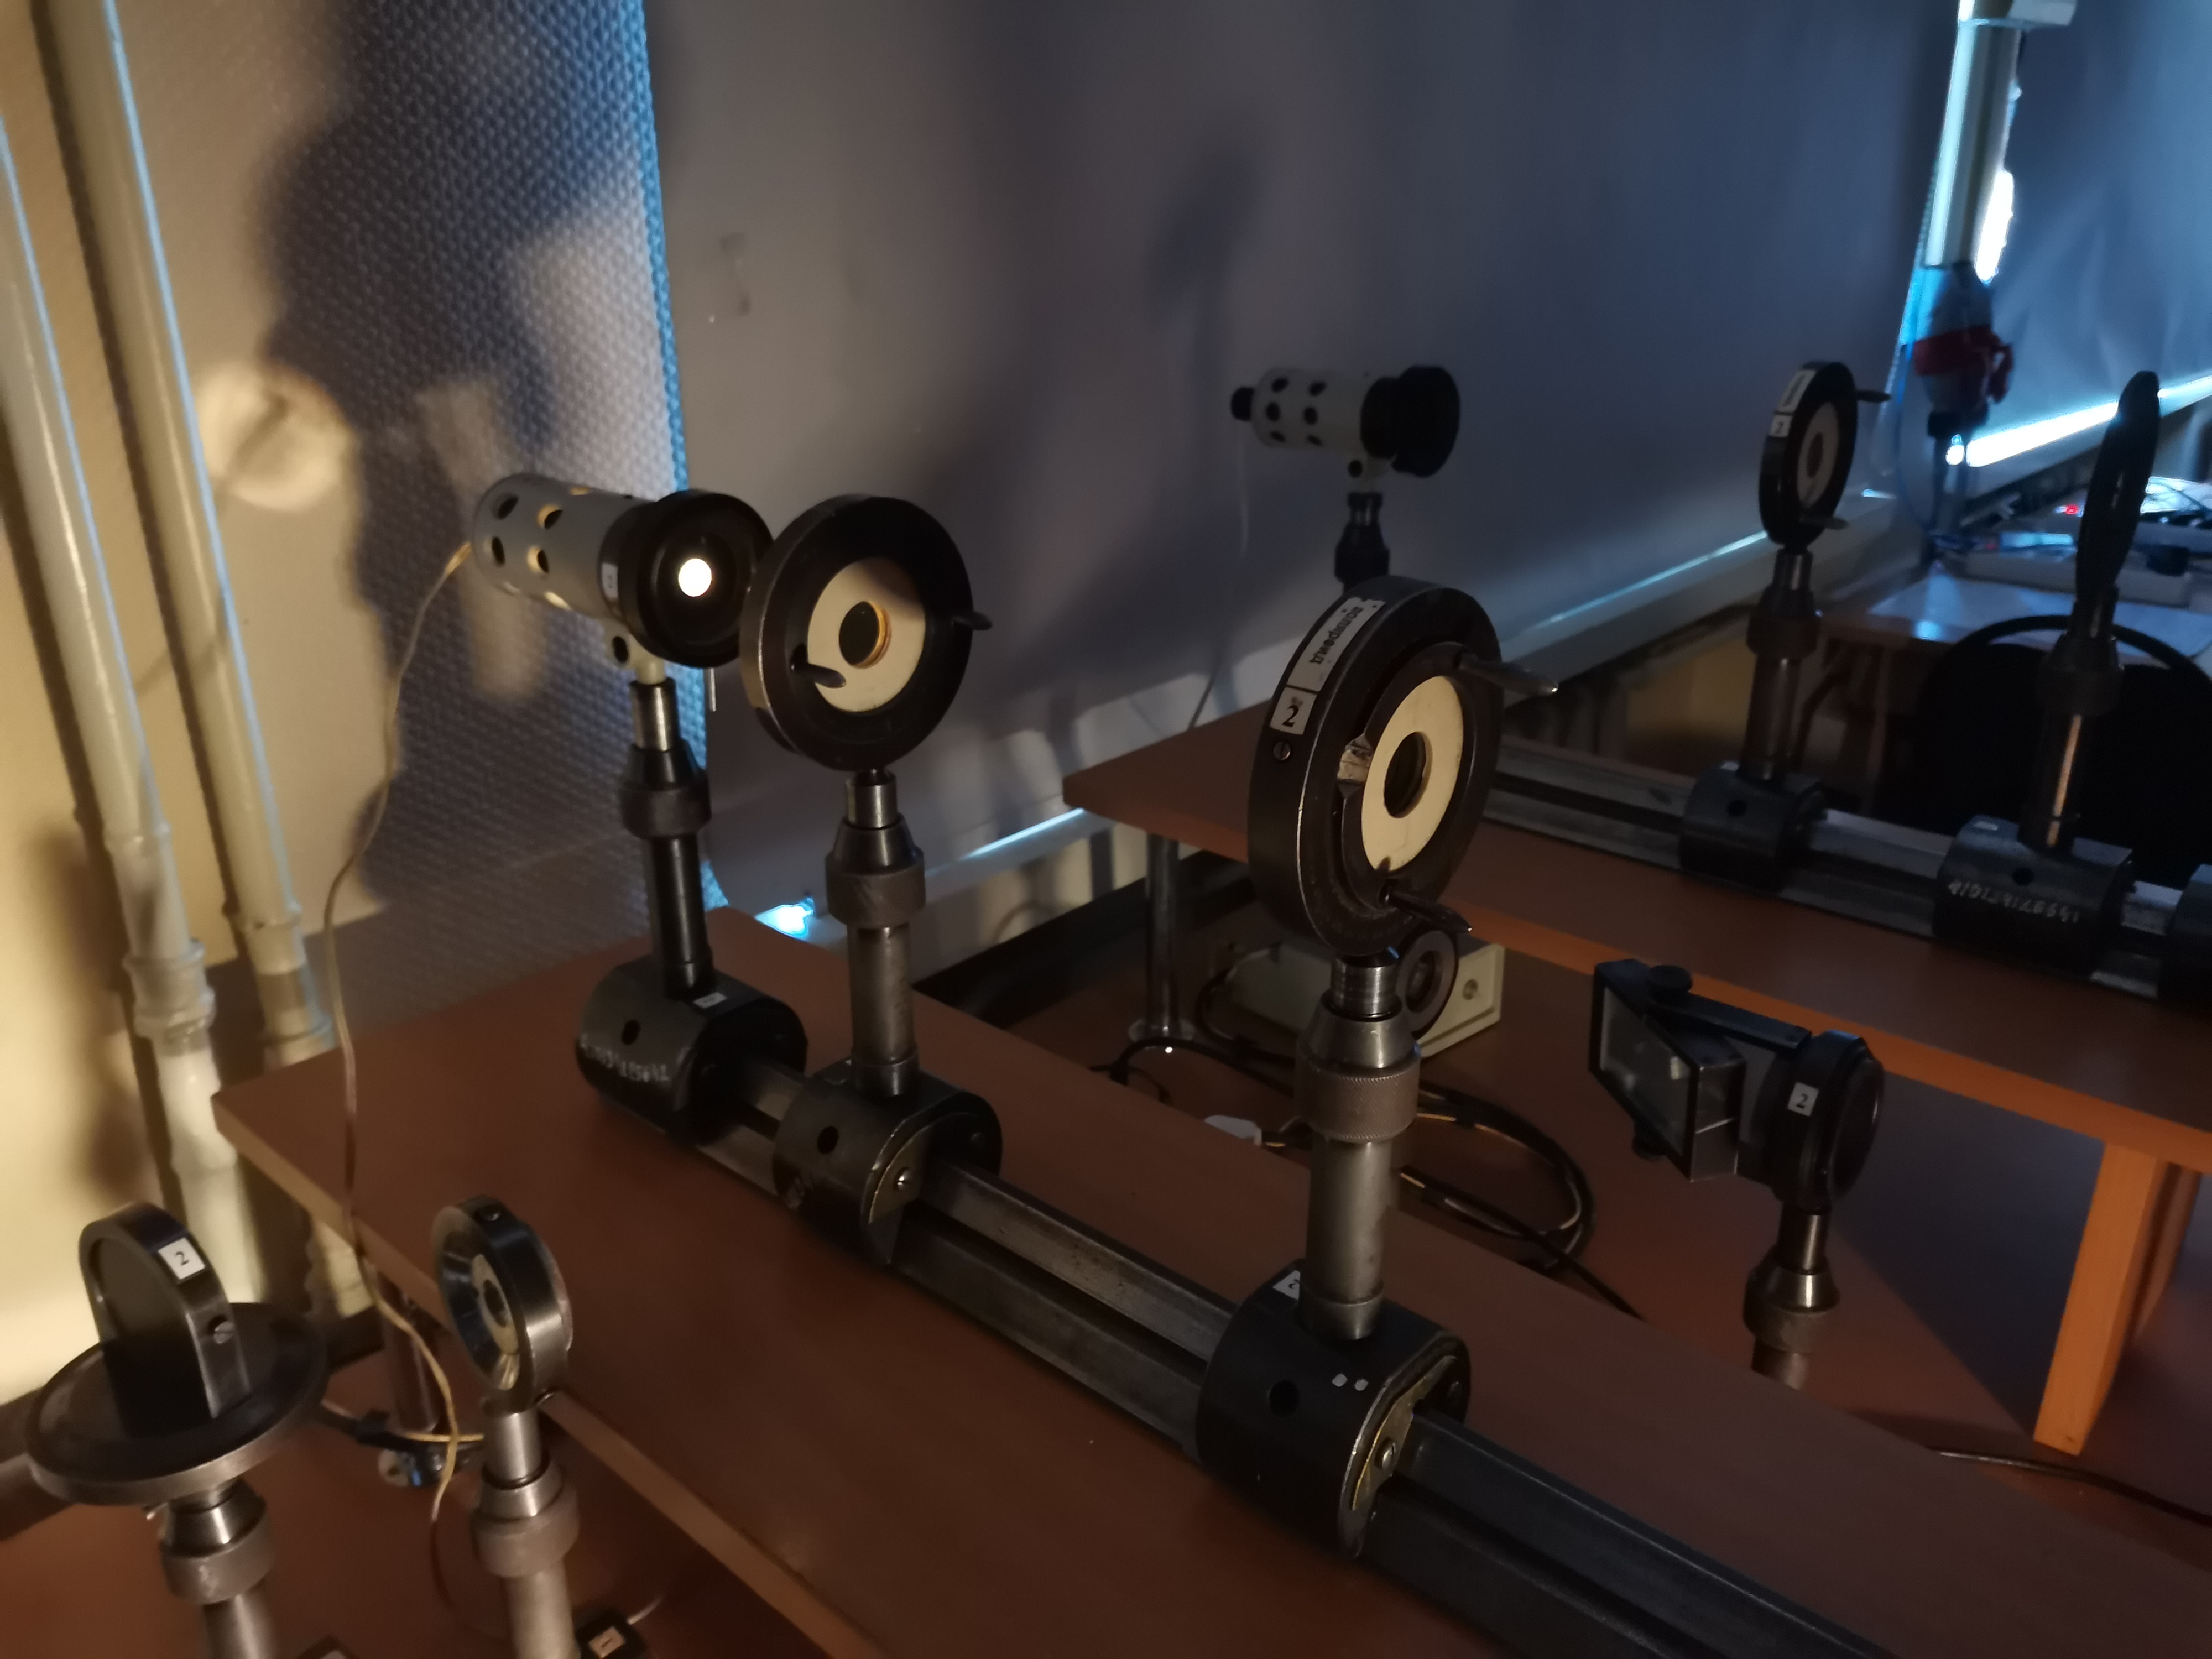
\includegraphics[width=1.1\textwidth]{images/2pol.jpg}
    \caption{The second polaroid.}
	\end{figure}
\end{minipage}
	\frametitle{The experiment photos}
}




\section{Brewester}

\frame{
And God said let there be light, and there was light
\begin{equation}
	\triangle E(\vc{r},t) - \mu_0 \varepsilon(\vc{r}) \frac{\partial^2}{\partial t^2} E(\vc{r}, t) = \mu_0 \frac{\partial^2}{\partial t^2} P_{in}(\vc{r},t)
\end{equation}
Which is solved as
\begin{equation*}
	E(\vc{r},t) = \frac{1}{2} E_0 e^{i(\beta y - \omega t)} + \const
\end{equation*}
And we assume:
\begin{equation*}
	E(\vc{r}, t) = A(t) E(s').
\end{equation*}	\frametitle{Theory behind the phenomenon}
}
\frame{
\begin{minipage}{0.35\textwidth}
    \begin{figure}[h]
    \centering
    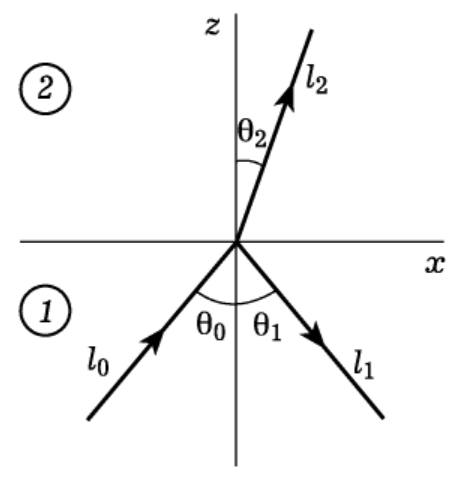
\includegraphics[width=1\textwidth]{images/brust.png}
    \caption{0 stands for a in-going wave, 1 stands for a transmitted wave, 2 stand for a reflected wave.}
    %\label{fig:}
\end{figure}
\end{minipage}
\hfill
\begin{minipage}{0.55\textwidth}
	 An incredible aspect describes the $\theta_p = \theta_0$ wich gives $\theta_0 + \theta_2 = \pi/2$.

	 With this and Snell's law we obtain:
	 \begin{equation}
	 	\tg \theta_p = \sqrt{\frac{\varepsilon_2}{\varepsilon_1}} = n.
	 \end{equation}
	 Where $\theta_p$ is the angle of polarization or \textit{Brewster's angle}.
\end{minipage}

	\frametitle{The main formula}
}
\frame{
\begin{minipage}{0.55\textwidth}
    \begin{figure}[h]
    \centering
    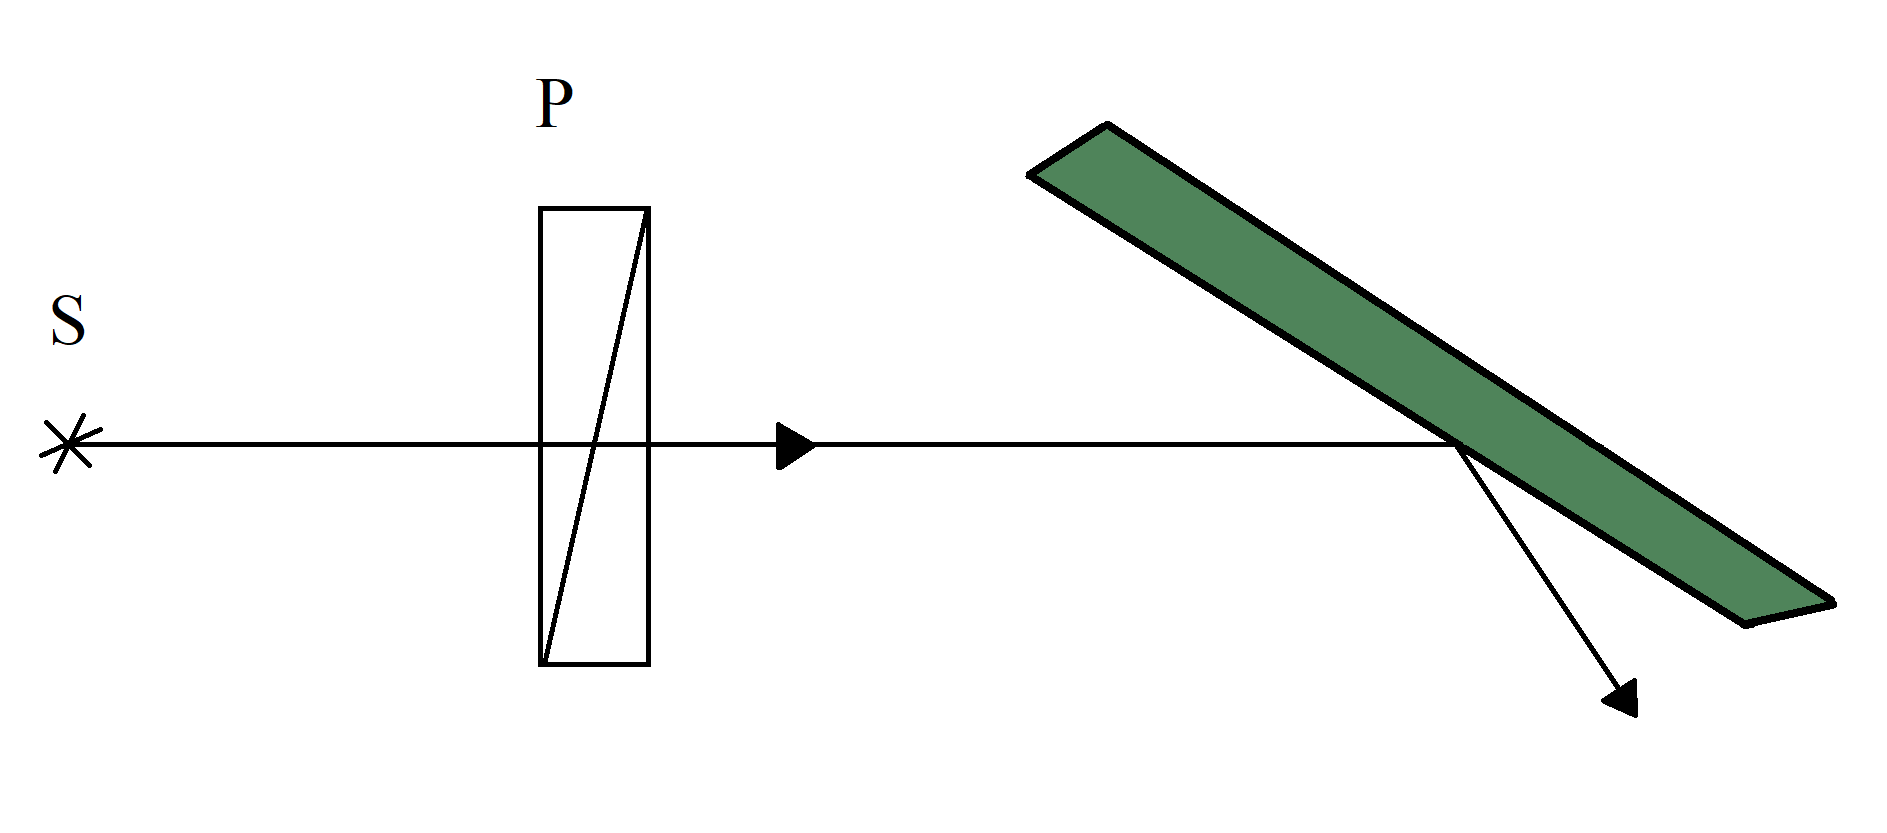
\includegraphics[width=1\textwidth]{images/ebonit.png}
    \caption{By rotating green ebonite plain we obtain several angles.}
    %\label{fig:}
\end{figure}
\end{minipage}
\hfill
\begin{minipage}{0.35\textwidth}
	\begin{center}
	\begin{tabular}{ |c|c|c| } 
		\hline
		name & $\theta_p$ & $\tg(\theta_p)$ \\
 		\hline
 		K & 240 & 1.73 \\ 
 		E & 237 & 1.54 \\ 
 		K & 237 & 1.54 \\ 
 		E & 238 & 1.60 \\ 
 		K & 236 & 1.48 \\ 
 		E & 239 & 1.66 \\ 
 		\hline
	\end{tabular}
	\end{center}
	The measurements were taken apart from each other.
\end{minipage}

	\frametitle{Our measurements}
}
\frame{
For the most beauty we assume that well is 1D, and the equastion:
\begin{equation}
	\frac{d A}{d t} = \frac{1}{2} v_g (\Gamma_{MD}G - i \Gamma_{MD} N_r)A,
\end{equation}
where $v_g = c/n_r$ is the speed of light in vacuum. And $\Gamma_{MD}G = g$ is so called gain coefficient.	\frametitle{Results}
}


\section{Stoletov}

\frame{
\begin{minipage}{0.55\textwidth}
    \begin{figure}[h]
    \centering
    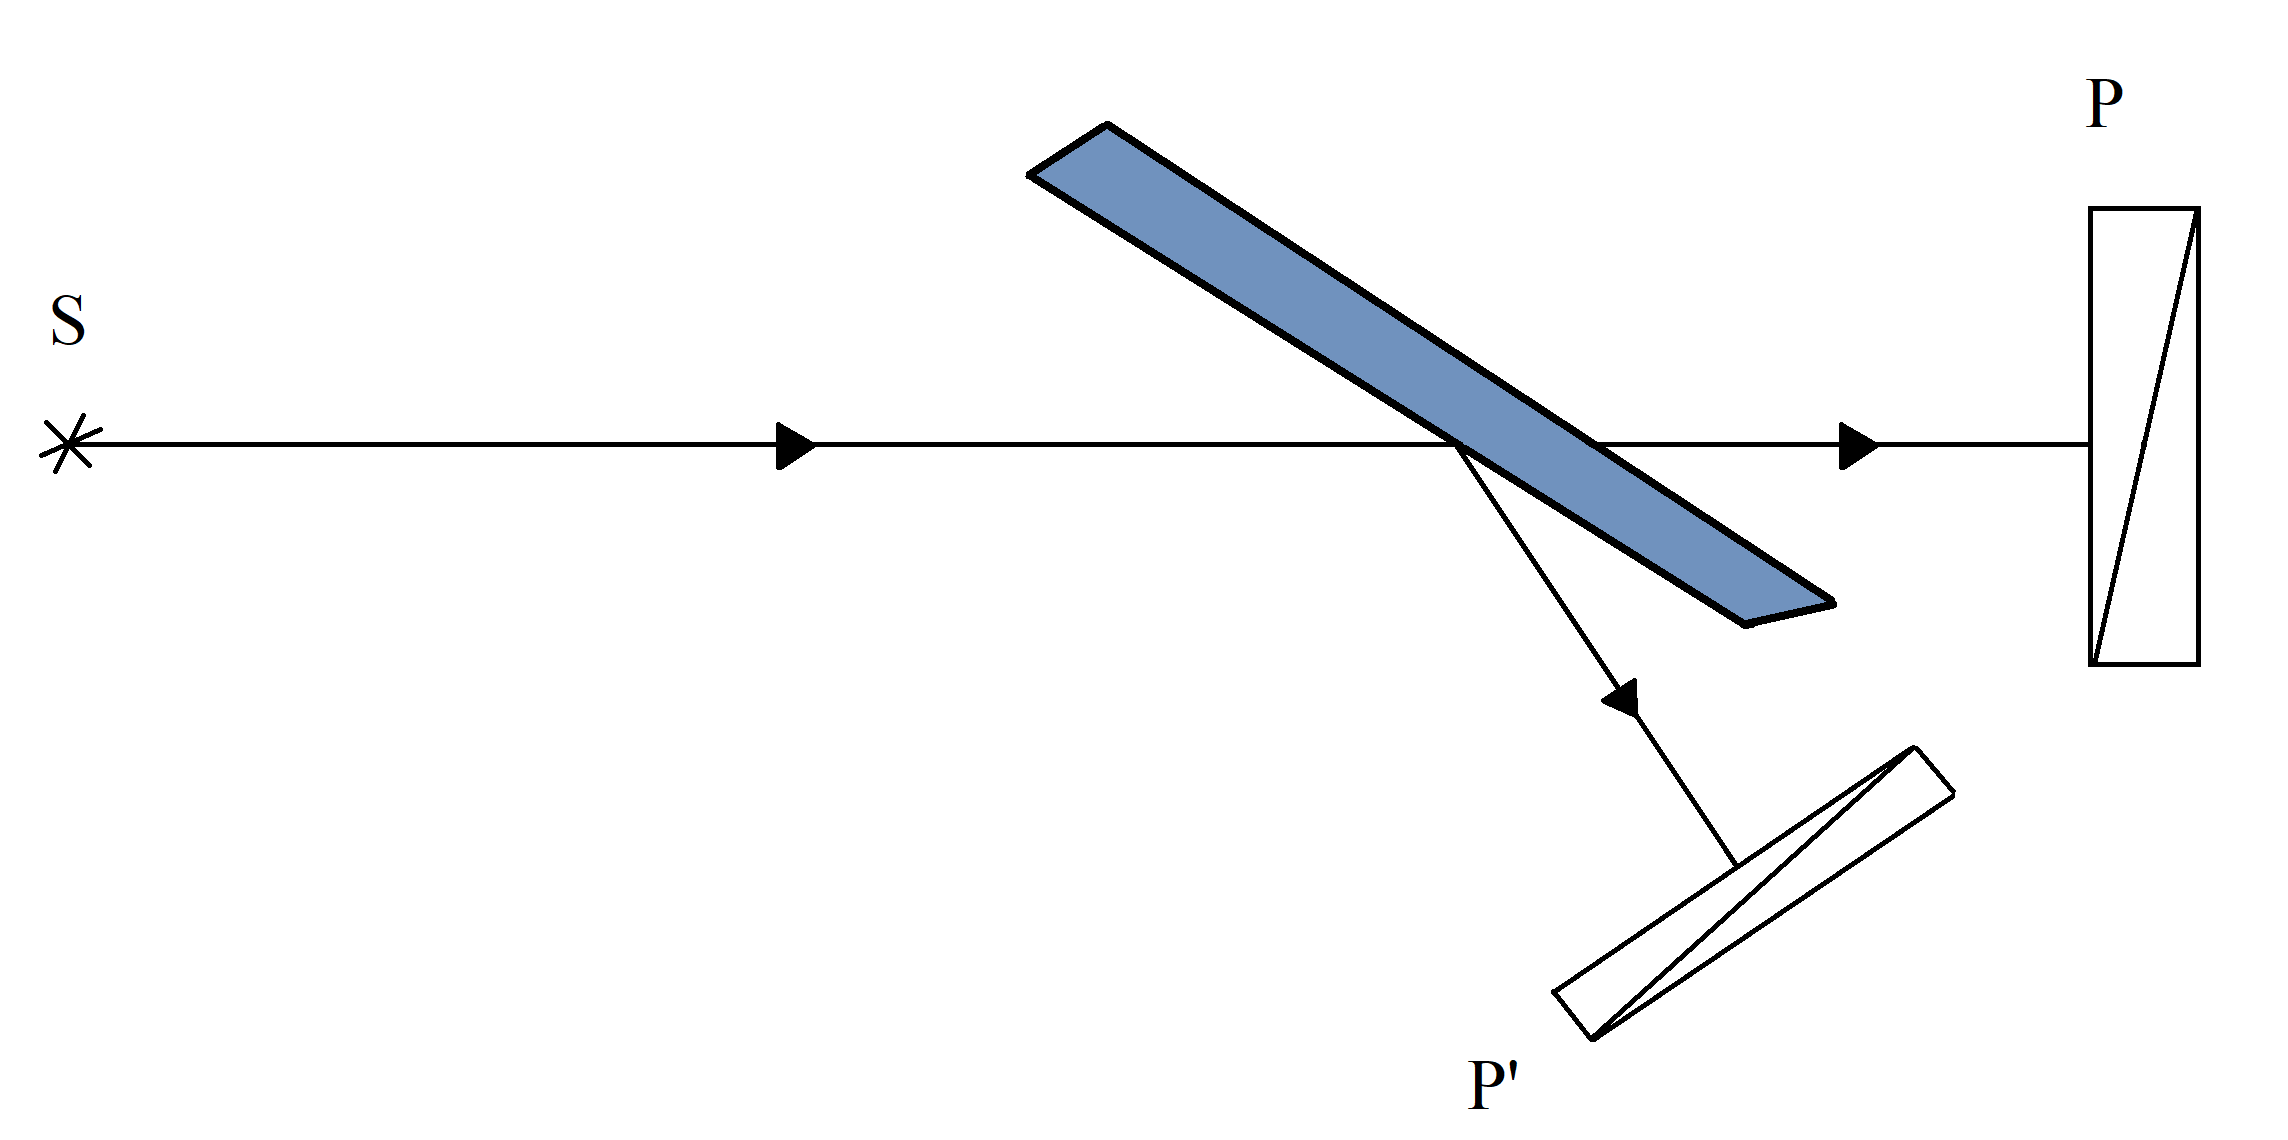
\includegraphics[width=1\textwidth]{images/stoletov.png}
    \caption{The beam goes right to the stack of glass (light blue) and then splits to two polaroids that we investigate before.}
    %\label{fig:}
\end{figure}
\end{minipage}
\hfill
\begin{minipage}{0.35\textwidth}
    Here we have to observe the with the polaroids from previous observation the direction of vector $E$.

    The polaroids were crossed when:
    \begin{align*}
    	P_1 \colon 98^\circ\\
    	P_2 \colon 26^\circ
    \end{align*}    
\end{minipage}
  \frametitle{Observation of reflected and rejected light}
}

\frame{
\begin{minipage}{0.55\textwidth}
    \begin{figure}[h]
    \centering
    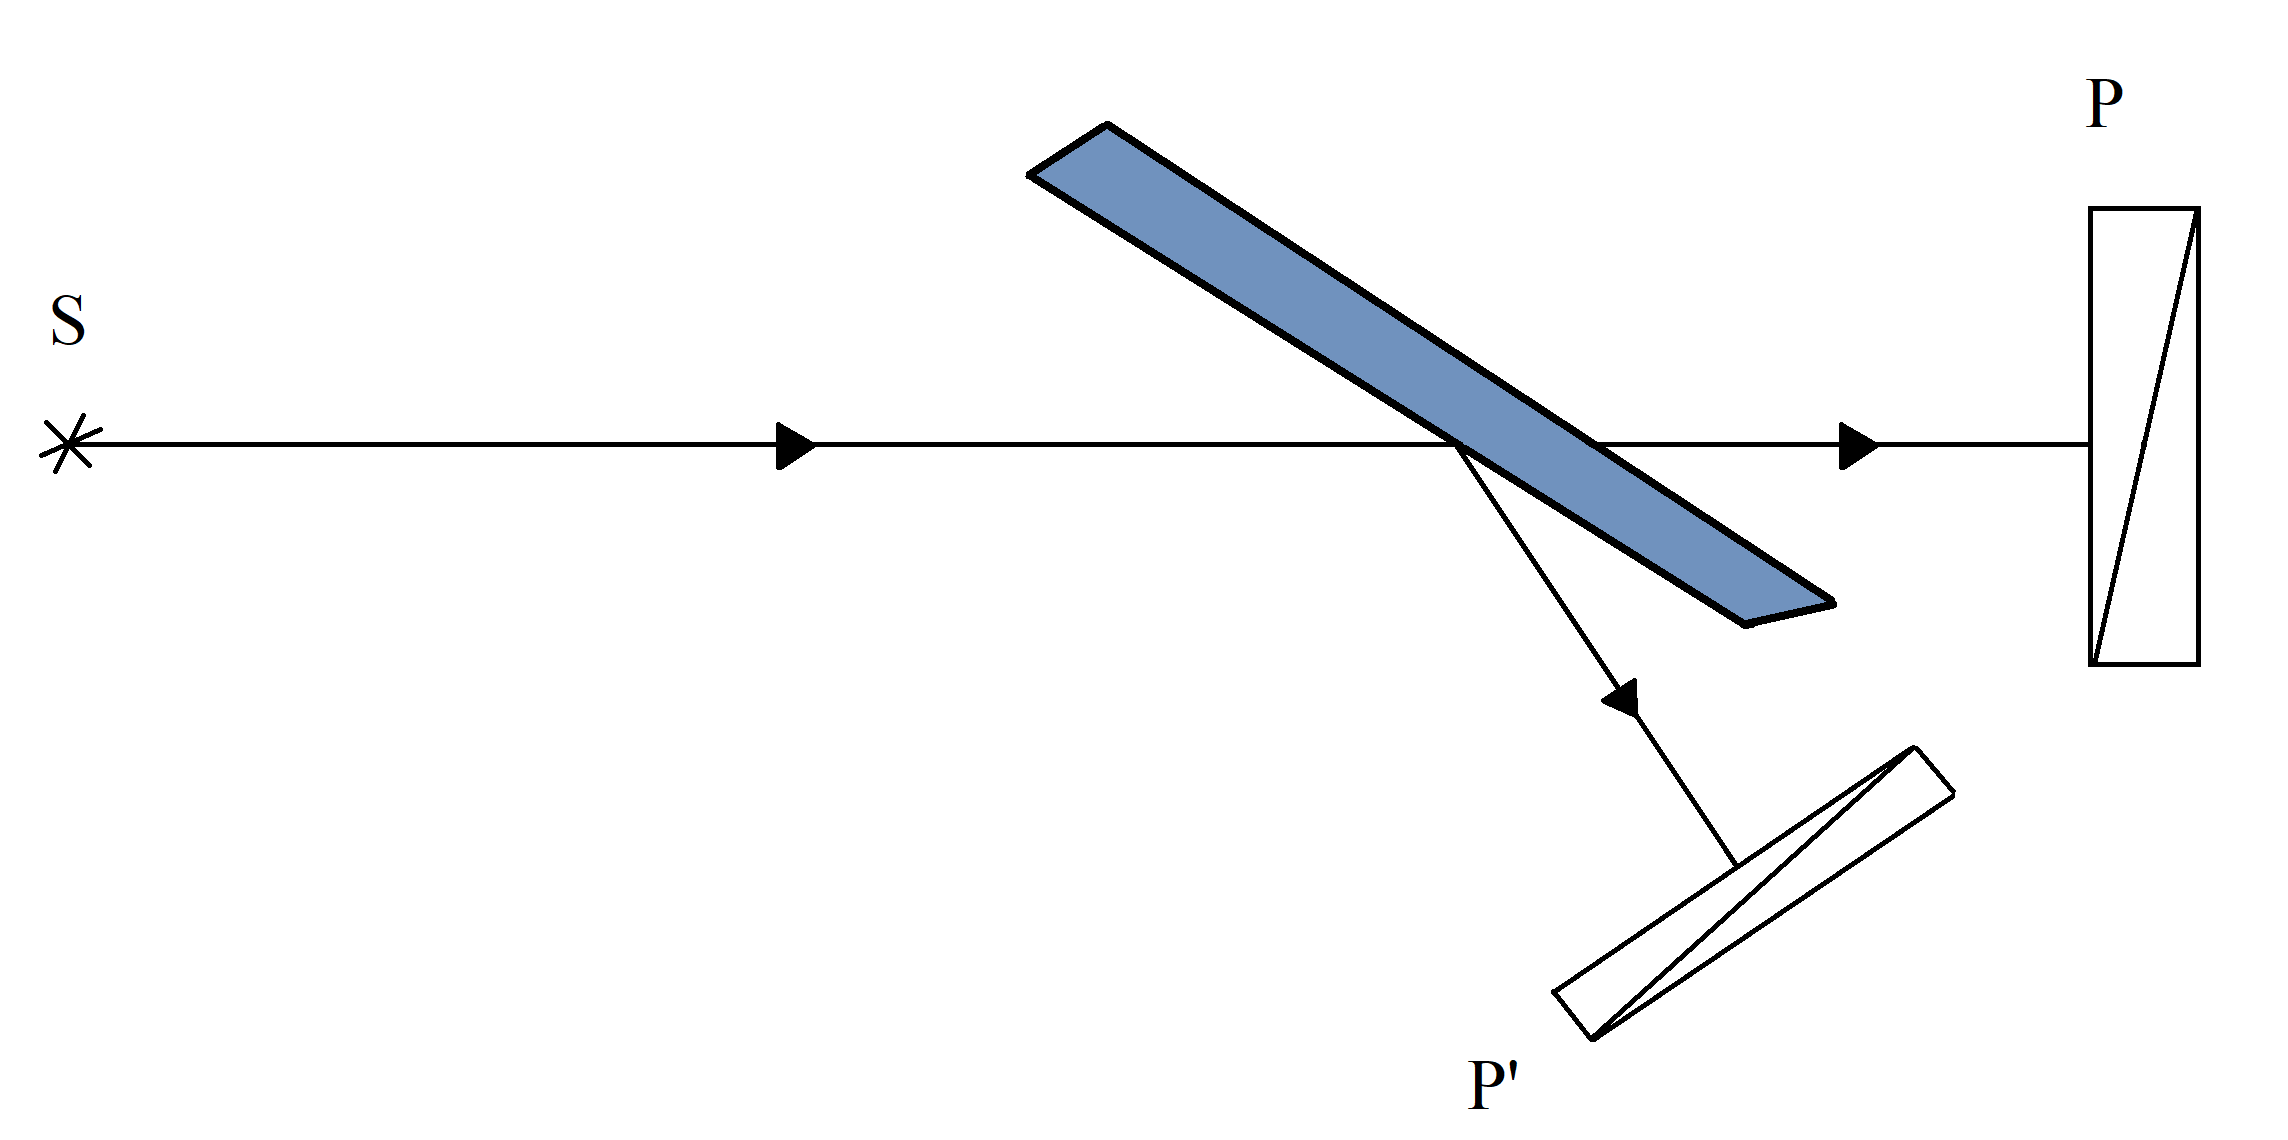
\includegraphics[width=1\textwidth]{images/stoletov.png}
    \caption{The beam goes right to the stack of glass (light blue) and then splits to two polaroids that we investigate before.}
    %\label{fig:}
\end{figure}
\end{minipage}
\hfill
\begin{minipage}{0.35\textwidth}
    So as was expected the reflected and transmitted light had an orthogonal $E$.

    The polaroids are crossed
    \begin{align*}
    	&P_1 \colon 98^\circ&\\
    	&P_2 \colon -265^\circ&
    \end{align*}
\end{minipage}
  \frametitle{Results}
}

\frame{
\begin{minipage}{0.55\textwidth}
    \begin{figure}[h]
    \centering
    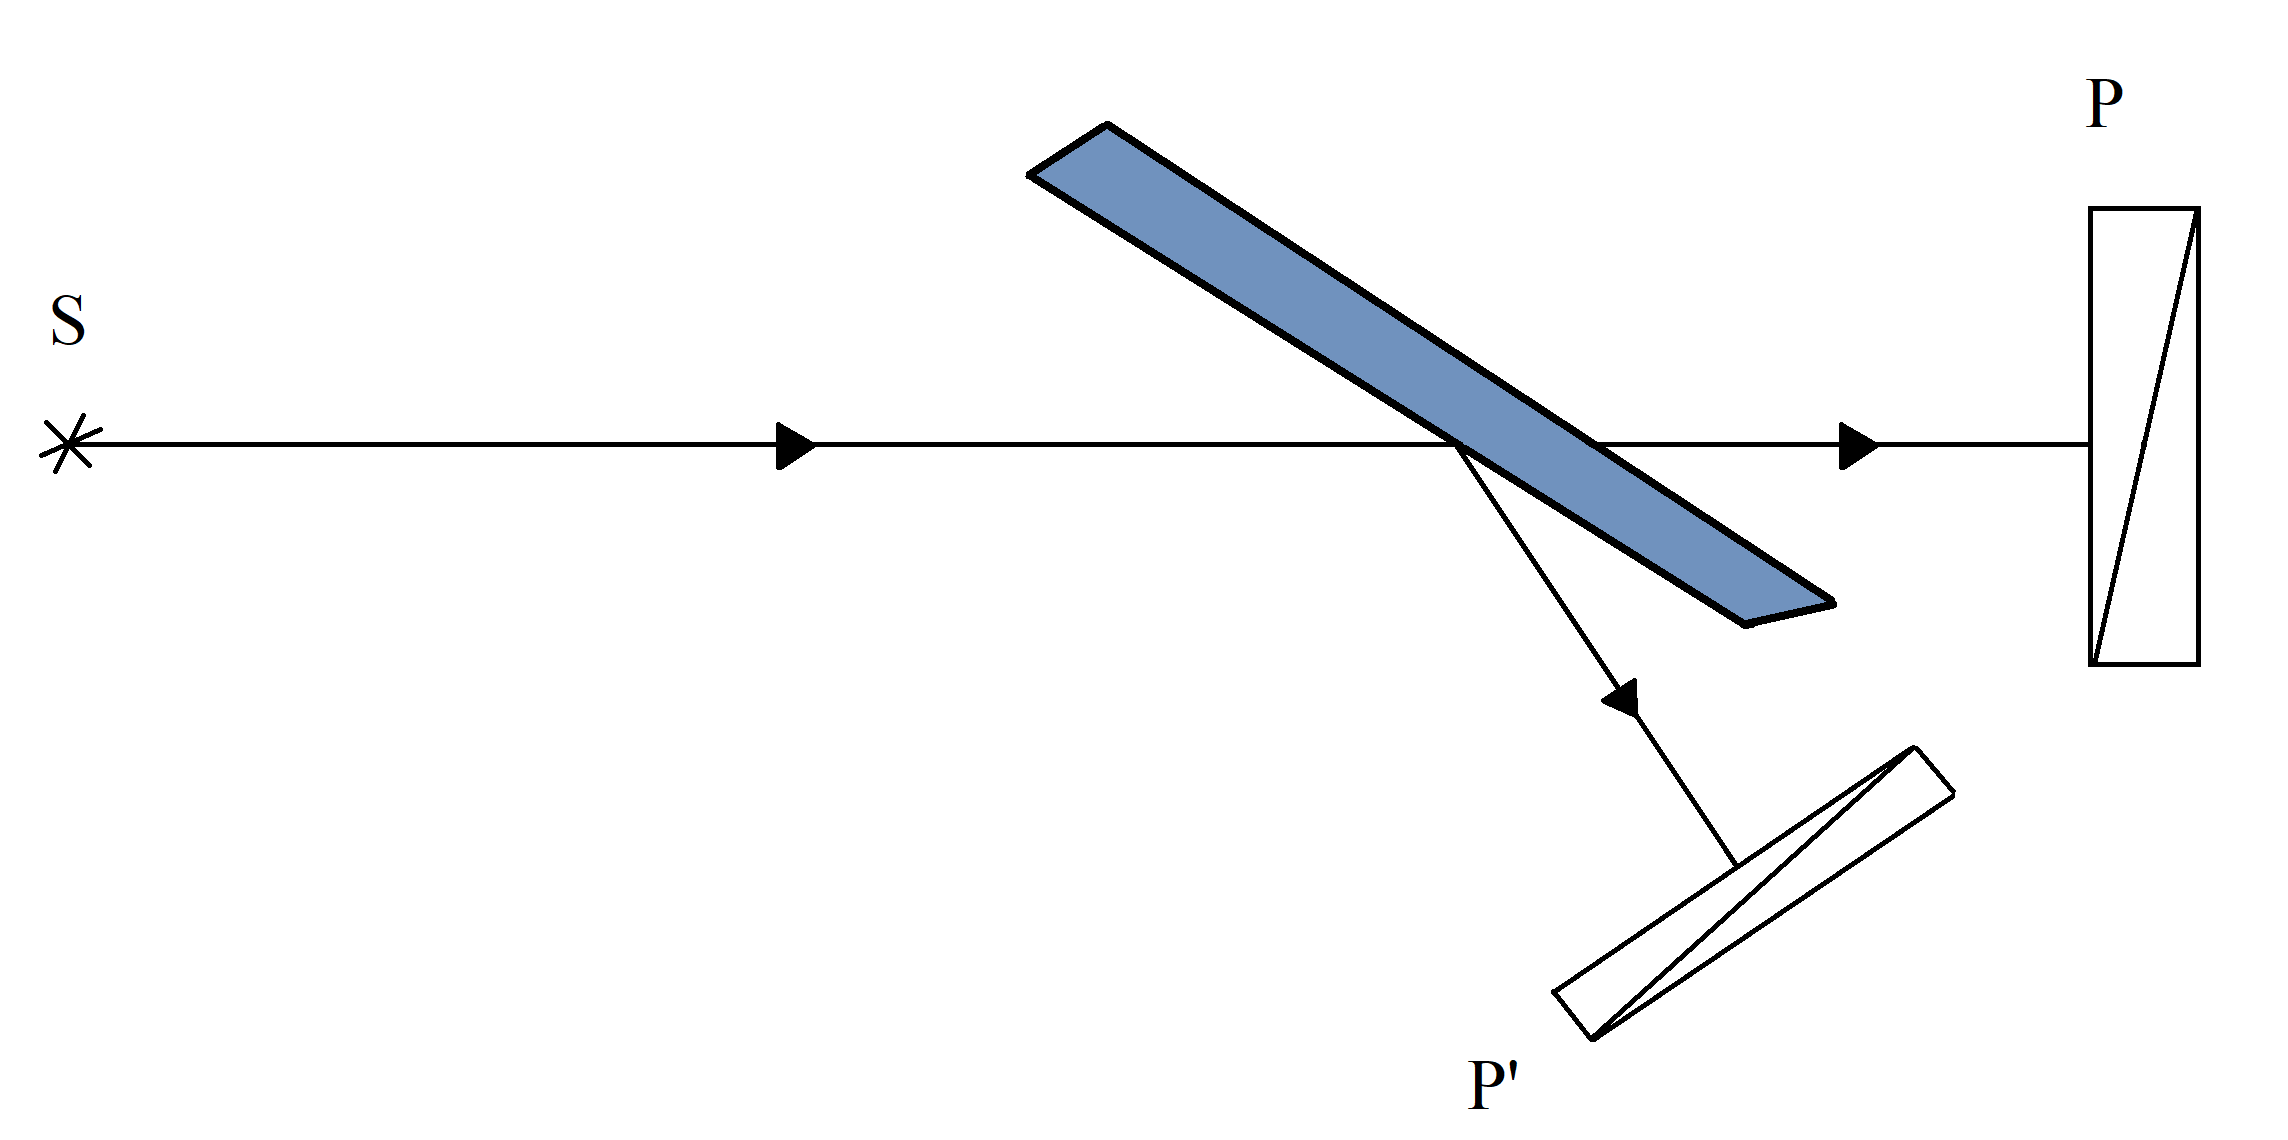
\includegraphics[width=1\textwidth]{images/stoletov.png}
    \caption{The beam goes right to the stack of glass (light blue) and then splits to two polaroids that we investigate before.}
    %\label{fig:}
\end{figure}
\end{minipage}
\hfill
\begin{minipage}{0.35\textwidth}
    Now we synchronize them by adding the period ($2 \pi$):
    \begin{align*}
        P_1 \colon 98^\circ\\
        P_2 \colon 95^\circ
    \end{align*}
    So the polaroids are again synchronized, as we expected it to be for transmitted and reflected light.
\end{minipage}
  \frametitle{Pleasant to look at results}
}


\section{2xRefracting}

\frame{
\begin{minipage}{0.55\textwidth}
    \begin{figure}[h]
    \centering
    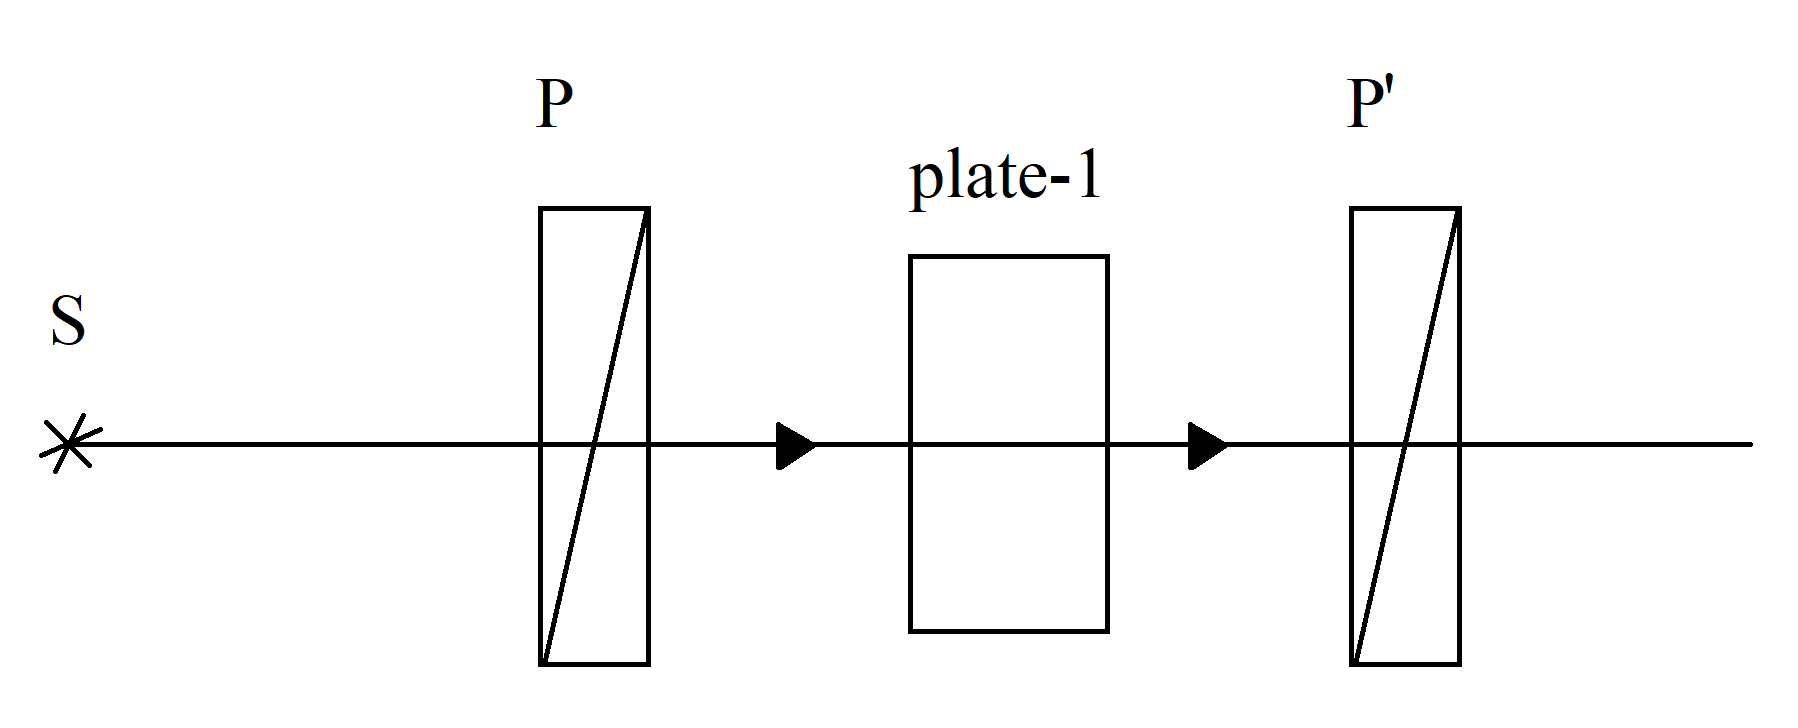
\includegraphics[width=1\textwidth]{images/crystplast.png}
    \caption{We add two crossed polaroids and the double refracting plate between them.}
    %\label{fig:}
\end{figure}
\end{minipage}
\hfill
\begin{minipage}{0.35\textwidth}
    So, when the polarizations match we observe maximum, and otherwise minimum of intensity.
    \begin{align*}
        \text{max} \colon 227^\circ\\
        \text{min} \colon 275^\circ
    \end{align*}
\end{minipage}
  \frametitle{Experimental set up 1}
}

\frame{
\begin{minipage}{0.55\textwidth}
    \begin{figure}[h]
    \centering
    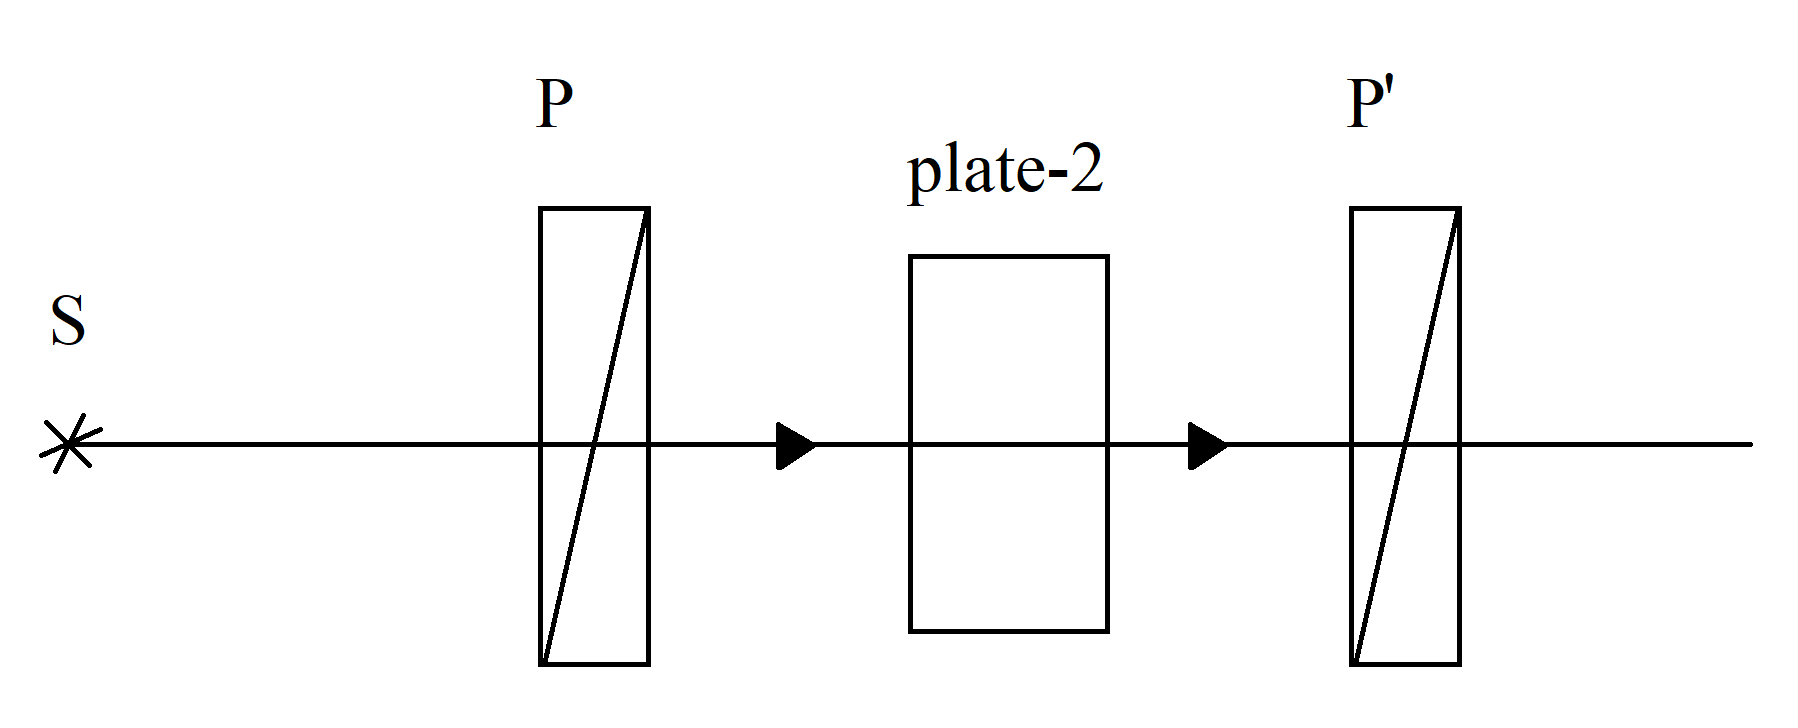
\includegraphics[width=1\textwidth]{images/crystplast2.png}
    \caption{We add two crossed polaroids and the double refracting plate between them.}
    %\label{fig:}
\end{figure}
\end{minipage}
\hfill
\begin{minipage}{0.35\textwidth}
    So, when the polarizations match we observe maximum, and otherwise minimum of intensity.
    \begin{align*}
        \text{max} \colon 86^\circ\\
        \text{min} \colon 43^\circ
    \end{align*}
\end{minipage}
  \frametitle{Experimental set up 2}
}


\section{Lambda}
\frame{
\begin{minipage}{0.55\textwidth}
    \begin{figure}[h]
    \centering
    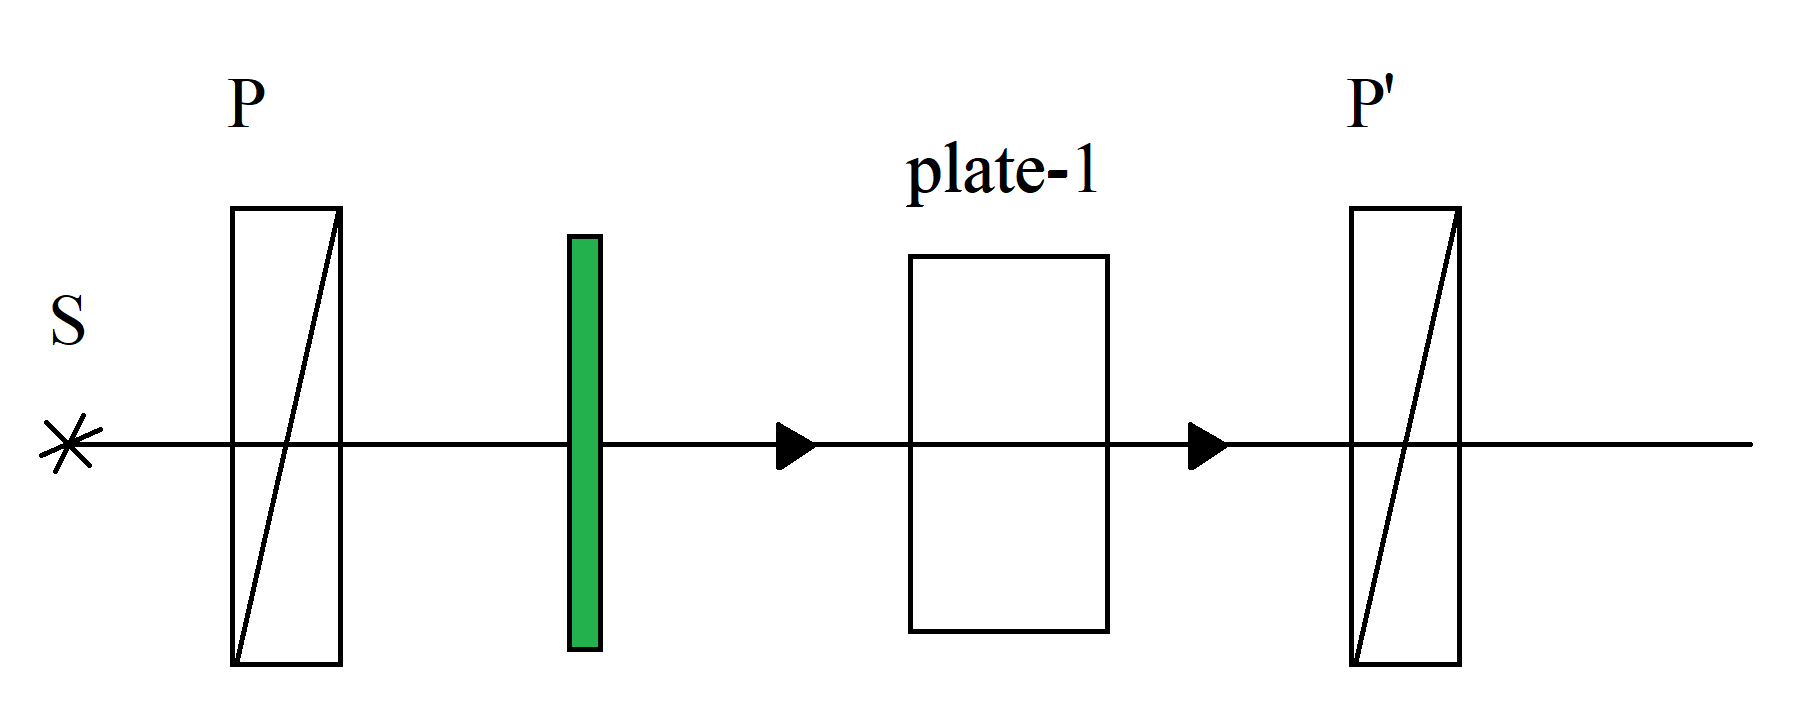
\includegraphics[width=1\textwidth]{images/greeeeeen.png}
    \caption{To the previous setup we add a green light-filter. And rotate the first polaraid so it is horizontal and the plate is  angled as $45^\circ$.}
    %\label{fig:}
\end{figure}
\end{minipage}
\hfill
\begin{minipage}{0.35\textwidth}
    By rotating the polaroid we obtain that plate-1 is $\lambda/4$, because it does not change the intensity, but it changes its polarization and creates phase difference $\pi/2$.
\end{minipage}
  \frametitle{Experimental set up}
}

\frame{


\begin{minipage}{0.45\textwidth}
\begin{figure}[h]
    \centering
    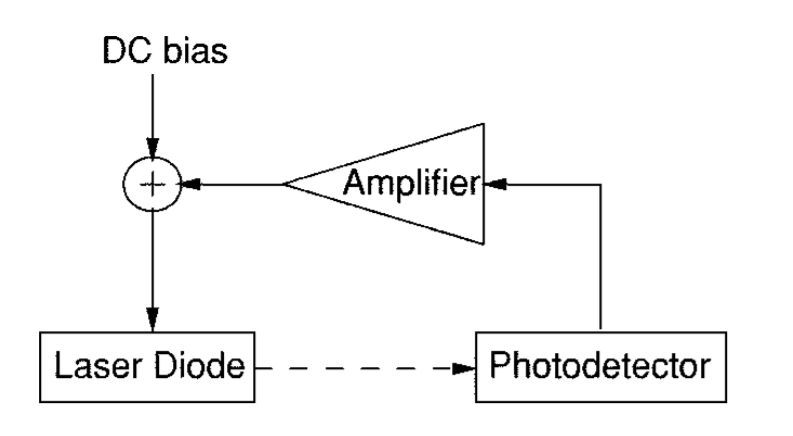
\includegraphics[width=1.1\textwidth]{images/55.png}
    %\caption{}
    %\label{fig:}
\end{figure}
\end{minipage}
\hfill
\begin{minipage}{0.45\textwidth}
\begin{itemize}
     \item DFB laser diod
     \item AR laser diod
     \item AlGaAs Single Mode Laser Diode
 \end{itemize} 
\end{minipage}

 \frametitle{Initial ideas}}


\end{document}



